\section{Sine exercise}

In this section we look at question 1 subquestion a, 
we want to add this extra explanation bla bla, and also 
note bla bla. \\

Out script is given by:
\lstinputlisting{sine.py}

Our script produces the following results, see Fig. \ref{fig:fig1},
compare with literature in Fig. \ref{fig:fig2}.


\begin{figure}[h!]
  \centering
  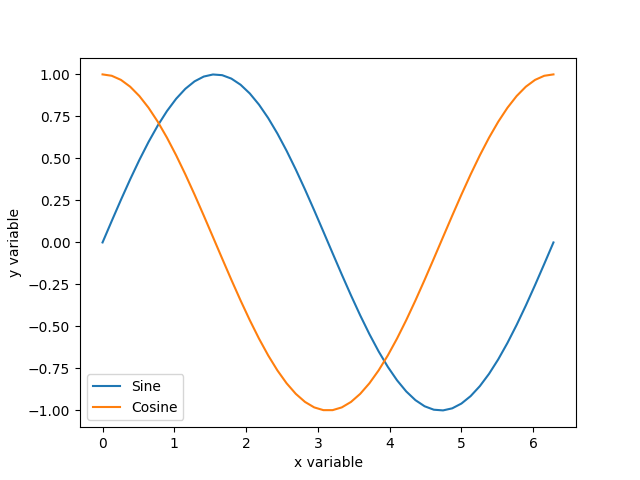
\includegraphics[width=0.9\linewidth]{./plots/sineplot.png}
  \caption{The result of our program, as can be seen the 
  sine and cosine are behaving exactly as expected, there 
  for we can conclude ....}
  \label{fig:fig1}
\end{figure}

\begin{figure}[h!]
  \centering
  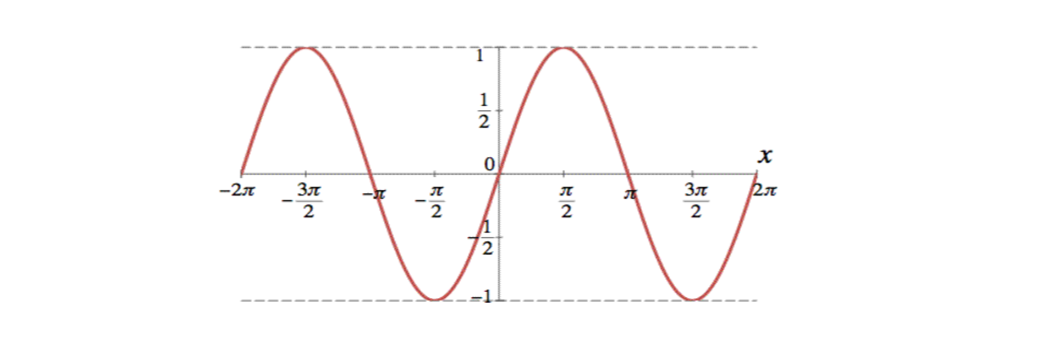
\includegraphics[width=0.9\linewidth]{./sine.png}
  \caption{Literature result, say something...}
  \label{fig:fig2}
\end{figure}
